\documentclass[12pt]{article}
\usepackage[left=25mm,right=25mm,top=30mm,bottom=30mm]{geometry}
\usepackage{amsmath} % math
\usepackage{amssymb} % math
\usepackage{graphicx} % to use \includegraphics{}
\usepackage{amsthm}
\usepackage{diagbox} % to make tables
\usepackage{kotex} % to use korean(hangul)
\usepackage{caption}
\usepackage{color}
\usepackage{setspace}
\usepackage{tabularx}
\usepackage{xfrac}
\usepackage{tikz}
\usepackage[firstpage]{draftwatermark}
\usepackage[hidelinks]{hyperref}
\usepackage[group-separator={,}]{siunitx} %si unit
% \usepackage[hangul]{kotex} 이걸로하면 Abstract, Contents 등이 전부 요약, 내용 등으로 바뀜.
\usepackage{listings}

\definecolor{codegreen}{rgb}{0,0.6,0}
\definecolor{codegray}{rgb}{0.5,0.5,0.5}
\definecolor{codepurple}{rgb}{0.58,0,0.82}
\definecolor{backcolour}{rgb}{0.95,0.95,0.92}
\lstdefinestyle{pstyle}{
	backgroundcolor=\color{backcolour},   
	commentstyle=\color{codegreen},
	keywordstyle=\color{magenta},
	numberstyle=\tiny\color{codegray},
	stringstyle=\color{codepurple},
	basicstyle=\footnotesize,
	breakatwhitespace=false,         
	breaklines=true,                 
	captionpos=b,                    
	keepspaces=true,                 
	numbers=left,                    
	numbersep=5pt,                  
	showspaces=false,                
	showstringspaces=false,
	showtabs=false,                  
	tabsize=2
}




\pagenumbering{roman} % \pagenumbering{다른거}나올때까지 roman으로 
%pagenumbering.
\renewcommand\thesection{\Roman{section}} % \section : In roman(I,II,III,...)
\renewcommand\thesubsection{\arabic{subsection}} % \subsection : In 
%arabic(1,2,3,...)

\usepackage{chngcntr}
\renewcommand\thesubsubsection{%
	\thesubsection.\arabic{subsubsection}%
}
\usepackage{titlesec}
\titlelabel{\thetitle.\quad}
%subsubsection에 점이 두 개씩 찍히는 것을 막고,
%점이 문단 번호에만 찍히도록 수정.

\usepackage{tocloft}%
\setlength{\cftsecnumwidth}{3em}% 
\setlength{\cftsubsecnumwidth}{1em}%
\setlength{\cftsubsubsecnumwidth}{2em}%
%toc의 여백 조정으로 VIII와 같은 번호가 제목과 겹치는 것을 방지

\SetWatermarkText{\includegraphics[angle=-45]{gshslatex_v2.jpg}}



\begin{document}
	
	{\bf \Huge Python Matplotlib로 그래프 그리기}
	
	\begin{LARGE}
		초보자를 위한 Matplotlib 활용하기
		\newline
		\newline
		\newline
		\newline
		\newline
	\end{LARGE} 


	
	\SetWatermarkAngle{0}
	\SetWatermarkText{
\includegraphics{gshs-tex-society-icon.jpg}}
	
	\begin{flushright}
		\vfill \LARGE 경기과학고등학교 \LaTeX 사용자 협회 울T
	\end{flushright}
	
	\clearpage
	%\tableofcontents
	\clearpage
	\pagenumbering{arabic}
	
	\setstretch{1.6}
	\section{왜 Python Matplotlib인가?}
	그래프를 그리는 비싼 프로그램들도 많다. 하지만 우린 돈이 없다. 그렇다고 그냥 엑셀로 그리면 폼나지 않는다. 우린 다행히 아주 조금 코딩을 할 수 있다. 최근에 나는 학생들이 활용할 수 있는 다양한 그래프를 그리기 위한 프로그램들을 사용해봤다.
	
	\begin{itemize}
		\item Gnuplot \textit{http://www.gnuplot.info/}
		\item Processing \textit{https://www.processing.org/}
		\item Python Matplotlib \textit{http://matplotlib.org/}
	\end{itemize}
	셋 다 대부분의 OS를 지원한다. Windows, Mac, Linux까지 지원한다. 여러가지 이유가 있지만 난 Matplotlib을 사용하려 한다. 파이썬이 처음이라고? 그래도 괜찮다. 아주 간단하다.
	
	\clearpage
	
	\section{파이썬 IDE 설치하고 첫 그래프 그리기}
		\subsection{파이썬 IDE}
			Matplotlib는 파이썬의 라이브러리이다. 사용하려면 당연히 파이썬을 설치해야 한다. 아주 하드하게 파이썬만 깔고 텍스트에디터에서 코딩해 저장한 다음 콘솔에서 실행할 수 있다. 하지만 난 IDE를 사용할 것을 추천한다. 여러모로 실행까지 편하다. 내가 사용해 본 IDE는 2개다.
			\begin{itemize}
				\item Anaconda \textit{https://www.continuum.io/downloads}
				\item Canopy \textit{https://www.enthought.com/products/canopy/}
			\end{itemize}
			두 개 중 하나를 받아 설치하자. 사용법은 DEV C++이나 Code block과 거의 비슷하다. 참고로 난 Canopy를 사용하고 있다.
			\subsubsection{Canopy 설치하기}
				Canopy 설치하기
			\clearpage
			\subsubsection{Canopy 둘러보기}
				Canopy 실행한 다음에 \textit{Edit}를 선택하면 빈 화면이 나온다. 
				\begin{figure}[h]
					\begin{center}
						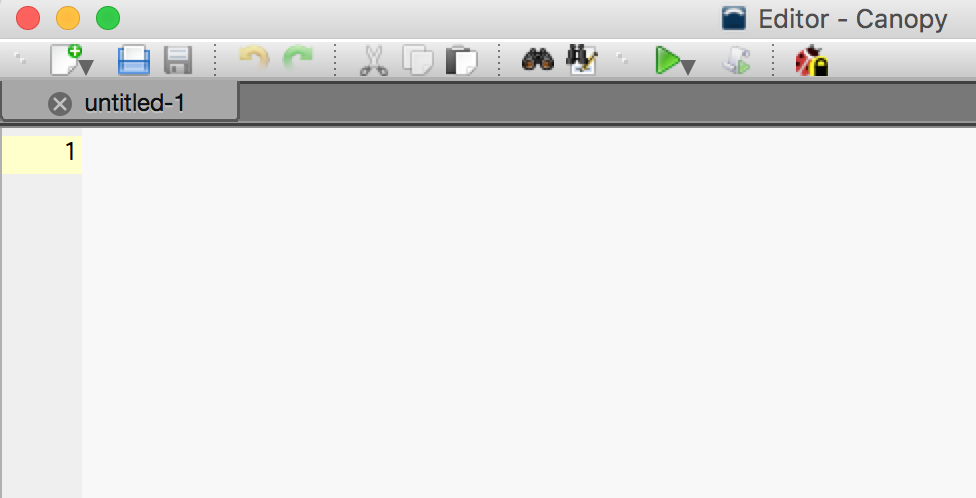
\includegraphics[height=7cm]{./images/2_2_b.png}
					\end{center}
				\end{figure}
				\\ 이제 코드를 입력하고 실행할 준비가 끝났다.
		\clearpage
		\subsection{Hello World!!}
			이제 첫번째 그래프를 그려볼 차례입니다. 보통 코딩을 배울 때 첫 프로그램은 항상 Hello World입니다. 하지만 그래프가 목표인 우리는 (0,0)과 (1,1)을 잇는 직선을 그려봅시다.\newline
			\subsubsection{코드 작성}
				\begin{lstlisting}[style=pstyle, language=Python, caption=first graph]
				import matplotlib.pyplot as plt
				
				plt.plot([0,1],[0,1])
				plt.show()\end{lstlisting}
				실제 Canopy 화면에 다음과 같이 입력하고 상단 메뉴 바에서 \textit{Run} - \textit{Run File}을 클릭하면 작성한 코드가 실행된다. 또는 단축키를 사용해도 좋다. 맥에서는 \textit{command+R}이다.
				\begin{figure}[h]
					\begin{center}
						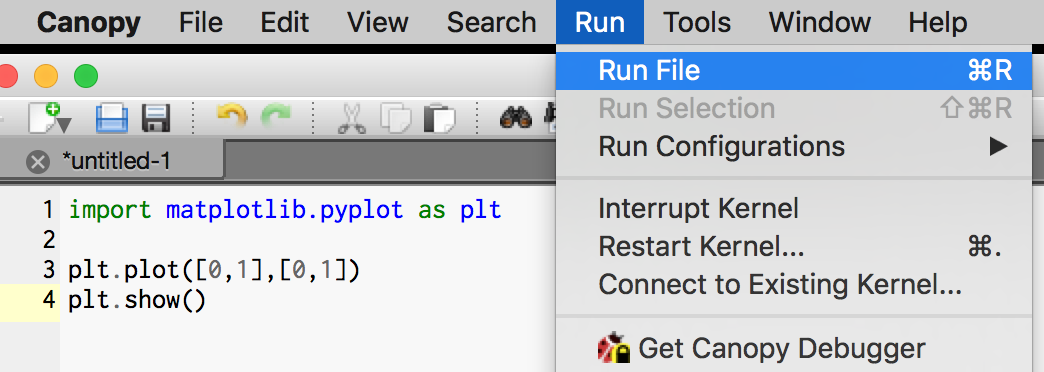
\includegraphics[height=5cm]{./images/2_2_c.png}
					\end{center}
				\end{figure}
			
			\clearpage
			\subsubsection{그래프 결과보기}
				\begin{figure}[h]
					\begin{center}
						\includegraphics[width=8cm]{./images/figure_1.pdf}
					\end{center}
				\end{figure}
				
			\subsubsection{그래프 저장하기}
				그래프는 여러 파일 형태로 저장할 수 있다. 일반적인 그림파일 형태(*.jpg, *.png 등)로 저장할 수 있다. 이렇게 저장한 파일은 어느 프로그램이나 쉽게 활용할 수 있지만 비트맵 형태의 파일이기때문에 확대를 하면 깨져보인다. 하지만 벡터파일 형태(*.pdf 등)로 저장해 활용하면 아무리 확대를 해도 깨지지 않고 깔끔하게 출력되거나 표시되는 것을 볼 수 있다.
				\begin{figure}[h]
					\begin{center}
						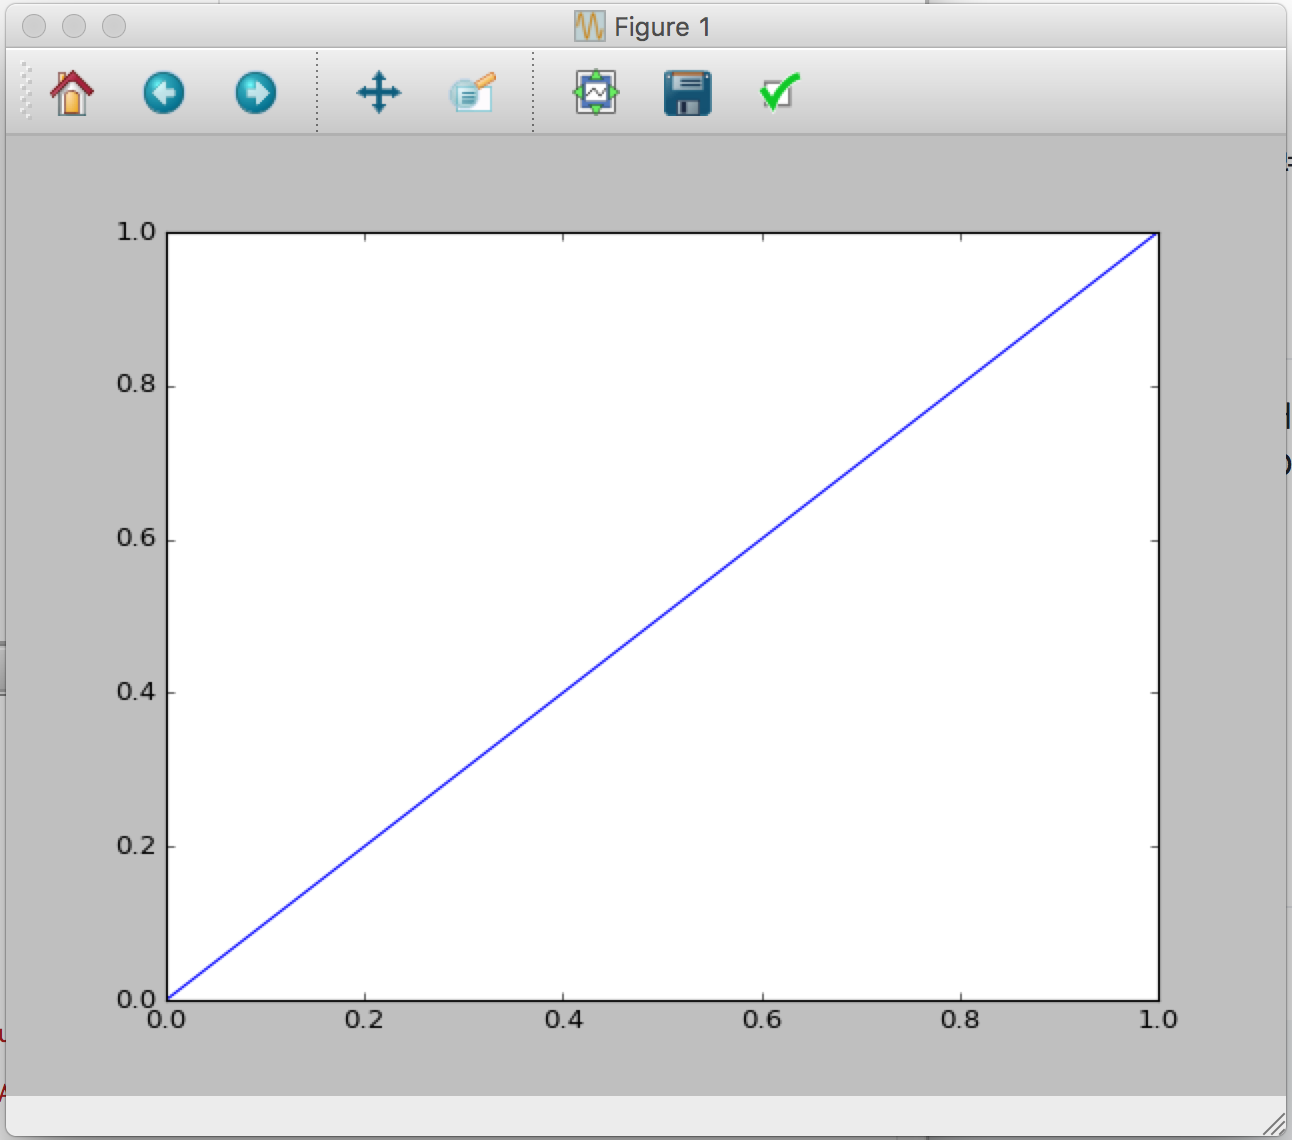
\includegraphics[height=5cm]{./images/3_3_a.png}
						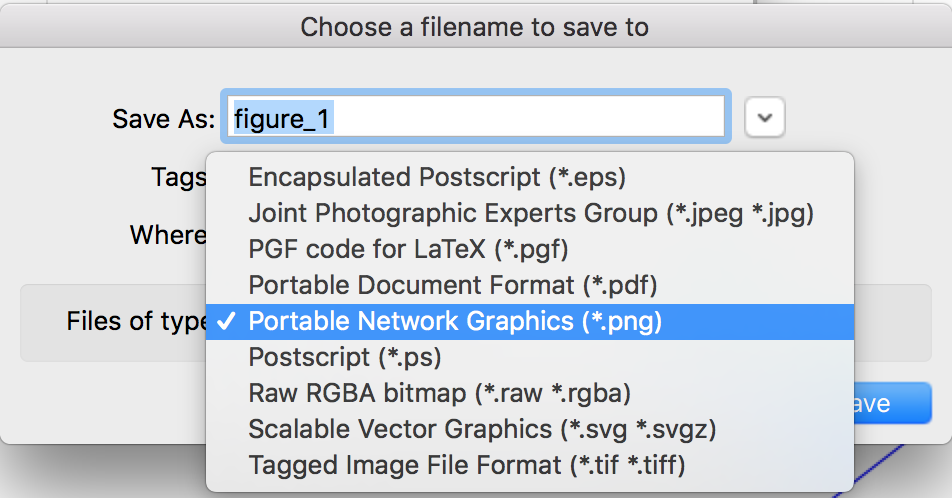
\includegraphics[height=5cm]{./images/3_3_b.png}
					\end{center}
				\end{figure}
				\\ 상단에 그래픽 아이콘 중 디스켓 모양을 클릭하면 파일을 저장할 수 있고, 파일 타입을 선택해 jpg나 png, pdf 등을 선택할 수 있다.
			
	\section{점으로 그래프 그리기}
		\subsection{x축과 y축 Label}
			앞에서 그렸던 그래프에 좌표를 다르게 바꾸고 축 라벨을 입력해보자.
			\subsubsection{코드 작성}
			\begin{lstlisting}[style=pstyle, language=Python, caption=axis label]
			import matplotlib.pyplot as plt
			
			plt.plot([0,60],[0,73])
			plt.xlabel('t[s]')
			plt.ylabel('x[m]')
			plt.show()\end{lstlisting}
			\subsubsection{그래프 결과보기}
			\begin{figure}[h]
				\begin{center}
					\includegraphics[width=10cm]{./images/figure_1.pdf}
				\end{center}
			\end{figure}
		
		\clearpage
		\subsection{3개의 점을 각각 연결한 그래프}
		점을 추가해보자. (0, 0), (60, 73.2), (84, 146.4) 세 점을 각각 연결해 그린다.
			\subsubsection{코드 작성}
			\begin{lstlisting}[style=pstyle, language=Python, caption=3 point]
			import matplotlib.pyplot as plt
			
			plt.plot([0,60,84],[0,73.2,146.4])
			plt.xlabel('t[s]')
			plt.ylabel('x[m]')
			plt.show()\end{lstlisting}
			\subsubsection{그래프 결과보기}
			\begin{figure}[h]
				\begin{center}
					\includegraphics[width=10cm]{./images/figure_2.pdf}
				\end{center}
			\end{figure}
		
		\clearpage
		\subsection{2개의 직선 그래프}
			직선을 하나 더 추가해보자.
			\subsubsection{코드 작성}
			\begin{lstlisting}[style=pstyle, language=Python, caption=2 line]
			import matplotlib.pyplot as plt
			
			plt.plot([0,60,84],[0,73.2,146.4])
			plt.plot([0,84],[0,146.4])
			plt.xlabel('t[s]')
			plt.ylabel('x[m]')
			plt.show()\end{lstlisting}
			\subsubsection{그래프 결과보기}
			\begin{figure}[h]
				\begin{center}
					\includegraphics[width=10cm]{./images/figure_3.pdf}
				\end{center}
			\end{figure}		
		
		\clearpage
		\subsection{간단한 연산 활용}
			우리는 지금 파이썬 코딩을 통해 그래프를 그리고 있다. 점의 좌표를 지정할 때, 간단한 연산도 다음과 같이 가능하다.
			\subsubsection{코드 작성}
			\begin{lstlisting}[style=pstyle, language=Python, caption=simple operation]
			import matplotlib.pyplot as plt
			
			plt.axis([0,130,0,300])
			plt.plot([0,60,120],[0,1.22*60,3.05*60+1.22*60])
			plt.plot([0,120],[0,3.05*60+1.22*60])
			plt.xlabel('t[s]')
			plt.ylabel('x[m]')
			plt.show()\end{lstlisting}
			\subsubsection{그래프 결과보기}
			\begin{figure}[h]
				\begin{center}
					\includegraphics[width=10cm]{./images/figure_4.pdf}
				\end{center}
			\end{figure}
		
	\section{조금 더 그려보기}
		임의의 수식을 그래프로 나타내야 할 때가 많다. 함수를 그리는 것도 간단하다. 함수를 정의하고 사용하면 된다. 가장 간단한 y=x 그래프를 그려보자. 
		\subsection{직선 그리기}
		먼저 직선을 그려보자.
		\subsubsection{코드 작성}
		\begin{lstlisting}[style=pstyle, language=Python, caption=linear function]
		import numpy as np
		import matplotlib.pyplot as plt
		
		x = np.arange(0.,10.,0.01)
		y = x
		
		plt.plot(x,y)
		plt.show()\end{lstlisting}
		가로 축에 사용할 t의 범위를 \textit{arrange}를 이용해 정의했다. 0에서부터 10까지 0.01 간격으로 배열을 만들었다. 
		
		\clearpage
		\subsubsection{그래프 결과보기}
		\begin{figure}[h]
			\begin{center}
				\includegraphics[width=10cm]{./images/figure_5.pdf}
			\end{center}
		\end{figure}
	
		\subsection{sin 함수}
		sin 함수와  cos 함수를 그려보자.
		\subsubsection{코드 작성}
		\begin{lstlisting}[style=pstyle, language=Python, caption=simple operation]
		import numpy as np
		import matplotlib.pyplot as plt
		
		x = np.arange(0.,10.,0.01)
		y = np.sin(x)
		z = np.cos(x)
		
		plt.plot(x,y)
		plt.plot(x,z)
		
		plt.show()\end{lstlisting}
		\subsubsection{그래프 결과보기}
		\begin{figure}[h]
			\begin{center}
				\includegraphics[width=10cm]{./images/figure_6.pdf}
			\end{center}
		\end{figure}
	
		\subsection{subplot}
		
	\section{그래프 꾸미기}
		\subsection{title}
		\subsection{ticks}
		\subsection{log scale}
		\subsection{color}
		\subsection{line style}
		
\end{document}
